\documentclass[]{article}
\usepackage{lmodern}
\usepackage{amssymb,amsmath}
\usepackage{ifxetex,ifluatex}
\usepackage{fixltx2e} % provides \textsubscript
\ifnum 0\ifxetex 1\fi\ifluatex 1\fi=0 % if pdftex
  \usepackage[T1]{fontenc}
  \usepackage[utf8]{inputenc}
\else % if luatex or xelatex
  \ifxetex
    \usepackage{mathspec}
  \else
    \usepackage{fontspec}
  \fi
  \defaultfontfeatures{Ligatures=TeX,Scale=MatchLowercase}
\fi
% use upquote if available, for straight quotes in verbatim environments
\IfFileExists{upquote.sty}{\usepackage{upquote}}{}
% use microtype if available
\IfFileExists{microtype.sty}{%
\usepackage[]{microtype}
\UseMicrotypeSet[protrusion]{basicmath} % disable protrusion for tt fonts
}{}
\PassOptionsToPackage{hyphens}{url} % url is loaded by hyperref
\usepackage[unicode=true]{hyperref}
\hypersetup{
            pdftitle={Logistic-LASSO Breast Cancer Classification Task},
            pdfauthor={Ngoc Duong - nqd2000},
            pdfborder={0 0 0},
            breaklinks=true}
\urlstyle{same}  % don't use monospace font for urls
\usepackage[margin=1in]{geometry}
\usepackage{color}
\usepackage{fancyvrb}
\newcommand{\VerbBar}{|}
\newcommand{\VERB}{\Verb[commandchars=\\\{\}]}
\DefineVerbatimEnvironment{Highlighting}{Verbatim}{commandchars=\\\{\}}
% Add ',fontsize=\small' for more characters per line
\usepackage{framed}
\definecolor{shadecolor}{RGB}{248,248,248}
\newenvironment{Shaded}{\begin{snugshade}}{\end{snugshade}}
\newcommand{\KeywordTok}[1]{\textcolor[rgb]{0.13,0.29,0.53}{\textbf{#1}}}
\newcommand{\DataTypeTok}[1]{\textcolor[rgb]{0.13,0.29,0.53}{#1}}
\newcommand{\DecValTok}[1]{\textcolor[rgb]{0.00,0.00,0.81}{#1}}
\newcommand{\BaseNTok}[1]{\textcolor[rgb]{0.00,0.00,0.81}{#1}}
\newcommand{\FloatTok}[1]{\textcolor[rgb]{0.00,0.00,0.81}{#1}}
\newcommand{\ConstantTok}[1]{\textcolor[rgb]{0.00,0.00,0.00}{#1}}
\newcommand{\CharTok}[1]{\textcolor[rgb]{0.31,0.60,0.02}{#1}}
\newcommand{\SpecialCharTok}[1]{\textcolor[rgb]{0.00,0.00,0.00}{#1}}
\newcommand{\StringTok}[1]{\textcolor[rgb]{0.31,0.60,0.02}{#1}}
\newcommand{\VerbatimStringTok}[1]{\textcolor[rgb]{0.31,0.60,0.02}{#1}}
\newcommand{\SpecialStringTok}[1]{\textcolor[rgb]{0.31,0.60,0.02}{#1}}
\newcommand{\ImportTok}[1]{#1}
\newcommand{\CommentTok}[1]{\textcolor[rgb]{0.56,0.35,0.01}{\textit{#1}}}
\newcommand{\DocumentationTok}[1]{\textcolor[rgb]{0.56,0.35,0.01}{\textbf{\textit{#1}}}}
\newcommand{\AnnotationTok}[1]{\textcolor[rgb]{0.56,0.35,0.01}{\textbf{\textit{#1}}}}
\newcommand{\CommentVarTok}[1]{\textcolor[rgb]{0.56,0.35,0.01}{\textbf{\textit{#1}}}}
\newcommand{\OtherTok}[1]{\textcolor[rgb]{0.56,0.35,0.01}{#1}}
\newcommand{\FunctionTok}[1]{\textcolor[rgb]{0.00,0.00,0.00}{#1}}
\newcommand{\VariableTok}[1]{\textcolor[rgb]{0.00,0.00,0.00}{#1}}
\newcommand{\ControlFlowTok}[1]{\textcolor[rgb]{0.13,0.29,0.53}{\textbf{#1}}}
\newcommand{\OperatorTok}[1]{\textcolor[rgb]{0.81,0.36,0.00}{\textbf{#1}}}
\newcommand{\BuiltInTok}[1]{#1}
\newcommand{\ExtensionTok}[1]{#1}
\newcommand{\PreprocessorTok}[1]{\textcolor[rgb]{0.56,0.35,0.01}{\textit{#1}}}
\newcommand{\AttributeTok}[1]{\textcolor[rgb]{0.77,0.63,0.00}{#1}}
\newcommand{\RegionMarkerTok}[1]{#1}
\newcommand{\InformationTok}[1]{\textcolor[rgb]{0.56,0.35,0.01}{\textbf{\textit{#1}}}}
\newcommand{\WarningTok}[1]{\textcolor[rgb]{0.56,0.35,0.01}{\textbf{\textit{#1}}}}
\newcommand{\AlertTok}[1]{\textcolor[rgb]{0.94,0.16,0.16}{#1}}
\newcommand{\ErrorTok}[1]{\textcolor[rgb]{0.64,0.00,0.00}{\textbf{#1}}}
\newcommand{\NormalTok}[1]{#1}
\usepackage{longtable,booktabs}
% Fix footnotes in tables (requires footnote package)
\IfFileExists{footnote.sty}{\usepackage{footnote}\makesavenoteenv{long table}}{}
\usepackage{graphicx,grffile}
\makeatletter
\def\maxwidth{\ifdim\Gin@nat@width>\linewidth\linewidth\else\Gin@nat@width\fi}
\def\maxheight{\ifdim\Gin@nat@height>\textheight\textheight\else\Gin@nat@height\fi}
\makeatother
% Scale images if necessary, so that they will not overflow the page
% margins by default, and it is still possible to overwrite the defaults
% using explicit options in \includegraphics[width, height, ...]{}
\setkeys{Gin}{width=\maxwidth,height=\maxheight,keepaspectratio}
\IfFileExists{parskip.sty}{%
\usepackage{parskip}
}{% else
\setlength{\parindent}{0pt}
\setlength{\parskip}{6pt plus 2pt minus 1pt}
}
\setlength{\emergencystretch}{3em}  % prevent overfull lines
\providecommand{\tightlist}{%
  \setlength{\itemsep}{0pt}\setlength{\parskip}{0pt}}
\setcounter{secnumdepth}{0}
% Redefines (sub)paragraphs to behave more like sections
\ifx\paragraph\undefined\else
\let\oldparagraph\paragraph
\renewcommand{\paragraph}[1]{\oldparagraph{#1}\mbox{}}
\fi
\ifx\subparagraph\undefined\else
\let\oldsubparagraph\subparagraph
\renewcommand{\subparagraph}[1]{\oldsubparagraph{#1}\mbox{}}
\fi

% set default figure placement to htbp
\makeatletter
\def\fps@figure{htbp}
\makeatother


\title{Logistic-LASSO Breast Cancer Classification Task}
\author{Ngoc Duong - nqd2000}
\date{3/25/2020}

\begin{document}
\maketitle

Data import and cleaning

\begin{Shaded}
\begin{Highlighting}[]
\NormalTok{breast_cancer_data =}\StringTok{ }\KeywordTok{read.csv}\NormalTok{(}\StringTok{"./breast-cancer-1.csv"}\NormalTok{)}

\NormalTok{bcdf =}\StringTok{ }\NormalTok{breast_cancer_data }\OperatorTok\StringTok{ }
\StringTok{  }\KeywordTok{mutate}\NormalTok{(}\DataTypeTok{diagnosis =} \KeywordTok{ifelse}\NormalTok{(diagnosis }\OperatorTok{==}\StringTok{ "M"}\NormalTok{,}\DecValTok{1}\NormalTok{,}\DecValTok{0}\NormalTok{)) }\OperatorTok\StringTok{ }
\StringTok{  }\NormalTok{dplyr}\OperatorTok{::}\KeywordTok{select}\NormalTok{(diagnosis, }\KeywordTok{everything}\NormalTok{()) }\OperatorTok\StringTok{ }
\StringTok{  }\NormalTok{dplyr}\OperatorTok{::}\KeywordTok{select}\NormalTok{(}\OperatorTok{-}\NormalTok{id, }\OperatorTok{-}\NormalTok{X)}
\end{Highlighting}
\end{Shaded}

Standardize design matrix (because although logistic is scale-invariant,
LASSO is not, this is to ensure comparability of estimates by these
different models)

\begin{Shaded}
\begin{Highlighting}[]
\NormalTok{pred_names =}\StringTok{ }\NormalTok{bcdf }\OperatorTok\StringTok{ }\NormalTok{dplyr}\OperatorTok{::}\KeywordTok{select}\NormalTok{(}\OperatorTok{-}\NormalTok{diagnosis) }\OperatorTok\StringTok{ }\KeywordTok{names}\NormalTok{() }\OperatorTok\StringTok{ }\KeywordTok{as.vector}\NormalTok{()}
\NormalTok{bcdf_x =}\StringTok{ }\OtherTok{NULL}

\ControlFlowTok{for}\NormalTok{ (i }\ControlFlowTok{in}\NormalTok{ pred_names) \{}
\NormalTok{col =}\StringTok{ }\NormalTok{(bcdf[,i] }\OperatorTok{-}\StringTok{ }\KeywordTok{mean}\NormalTok{(bcdf[,i]))}\OperatorTok{/}\KeywordTok{sd}\NormalTok{(bcdf[,i])}
\NormalTok{bcdf_x =}\StringTok{ }\KeywordTok{cbind}\NormalTok{(bcdf_x , col)}
\NormalTok{\}}

\KeywordTok{colnames}\NormalTok{(bcdf_x) <-}\StringTok{ }\KeywordTok{c}\NormalTok{(pred_names)}

\NormalTok{bcdf_fin =}\StringTok{ }\KeywordTok{cbind}\NormalTok{(bcdf[}\DecValTok{1}\NormalTok{], bcdf_x)}
\end{Highlighting}
\end{Shaded}

Investigate multicollinearity problem

\begin{Shaded}
\begin{Highlighting}[]
\NormalTok{p1 <-}\StringTok{ }\NormalTok{bcdf_fin }\OperatorTok\StringTok{ }\NormalTok{dplyr}\OperatorTok{::}\KeywordTok{select}\NormalTok{(}\OperatorTok{-}\NormalTok{diagnosis) }\OperatorTok\StringTok{  }\CommentTok{#filter only numeric variables}
\StringTok{  }\KeywordTok{cor}\NormalTok{() }\OperatorTok\StringTok{   }
\StringTok{  }\CommentTok{#compute correlation matrix}
\StringTok{  }\KeywordTok{ggcorrplot}\NormalTok{(.,}\DataTypeTok{ggtheme =}\NormalTok{ ggplot2}\OperatorTok{::}\NormalTok{theme_gray,}
             \DataTypeTok{colors =} \KeywordTok{c}\NormalTok{(}\StringTok{"#6D9EC1"}\NormalTok{, }\StringTok{"white"}\NormalTok{, }\StringTok{"#E46726"}\NormalTok{),}
             \DataTypeTok{tl.cex =} \DecValTok{6}\NormalTok{)}
\KeywordTok{ggsave}\NormalTok{(}\StringTok{"plot1.pdf"}\NormalTok{, p1, }\DataTypeTok{width =} \FloatTok{8.3}\NormalTok{, }\DataTypeTok{height =} \FloatTok{6.3}\NormalTok{) }
\CommentTok{#We can see that there are some very strong correlations between certain variables}
\end{Highlighting}
\end{Shaded}

Find correlation pairs that are above 0.85 to leave out of the dataset

\begin{Shaded}
\begin{Highlighting}[]
\CommentTok{#obtain list of variables that are correlated with one another whose correlation is at least 0.85}
\NormalTok{cor_var =}\StringTok{ }\NormalTok{bcdf_x }\OperatorTok\StringTok{ }
\StringTok{    }\KeywordTok{correlate}\NormalTok{() }\OperatorTok\StringTok{ }
\StringTok{    }\KeywordTok{stretch}\NormalTok{() }\OperatorTok\StringTok{ }
\StringTok{    }\KeywordTok{arrange}\NormalTok{(}\KeywordTok{desc}\NormalTok{(r)) }\OperatorTok\StringTok{ }
\StringTok{    }\KeywordTok{filter}\NormalTok{(r }\OperatorTok{>}\StringTok{ }\FloatTok{0.85}\NormalTok{) }\OperatorTok\StringTok{ }
\StringTok{    }\KeywordTok{slice}\NormalTok{(}\KeywordTok{which}\NormalTok{(}\KeywordTok{row_number}\NormalTok{() }\OperatorTok\StringTok{ }\DecValTok{2} \OperatorTok{==}\StringTok{ }\DecValTok{0}\NormalTok{)) }\OperatorTok\StringTok{ }
\StringTok{    }\KeywordTok{pivot_longer}\NormalTok{(x}\OperatorTok{:}\NormalTok{y) }\OperatorTok\StringTok{ }\NormalTok{dplyr}\OperatorTok{::}\KeywordTok{select}\NormalTok{(}\OperatorTok{-}\NormalTok{r,}\OperatorTok{-}\NormalTok{name) }\OperatorTok\StringTok{ }\KeywordTok{distinct}\NormalTok{(value) }

\CommentTok{#full data with response variable and predictors}
\NormalTok{full_data =}\StringTok{ }\KeywordTok{as_tibble}\NormalTok{(bcdf_fin) }\OperatorTok\StringTok{ }\NormalTok{dplyr}\OperatorTok{::}\KeywordTok{select}\NormalTok{(}\OperatorTok{-}\NormalTok{perimeter_mean, }\OperatorTok{-}\NormalTok{radius_mean, }\OperatorTok{-}\NormalTok{perimeter_worst, }\OperatorTok{-}\NormalTok{radius_worst, }\OperatorTok{-}\NormalTok{area_mean, }\OperatorTok{-}\NormalTok{area_worst, }\OperatorTok{-}\NormalTok{perimeter_se, }\OperatorTok{-}\NormalTok{radius_se, }\OperatorTok{-}\NormalTok{area_se, }\OperatorTok{-}\NormalTok{concave.points_mean, }\OperatorTok{-}\NormalTok{concavity_mean, }\OperatorTok{-}\NormalTok{texture_worst, }\OperatorTok{-}\NormalTok{texture_mean, }\OperatorTok{-}\NormalTok{compactness_worst, }\OperatorTok{-}\NormalTok{concave.points_worst, }\OperatorTok{-}\NormalTok{concavity_worst,}\OperatorTok{-}\NormalTok{compactness_mean) }

\CommentTok{#design matrix without intercept}
\NormalTok{Xmat_no_int =}\StringTok{ }\NormalTok{full_data }\OperatorTok\StringTok{ }\NormalTok{dplyr}\OperatorTok{::}\KeywordTok{select}\NormalTok{(}\OperatorTok{-}\NormalTok{diagnosis) }

\CommentTok{#design matrix with intercept}
\NormalTok{Xmat_int =}\StringTok{ }\NormalTok{Xmat_no_int }\OperatorTok\StringTok{ }\KeywordTok{mutate}\NormalTok{(}\DataTypeTok{intercept =} \DecValTok{1}\NormalTok{)}
\end{Highlighting}
\end{Shaded}

Looking at logistic regression results by glm

\begin{Shaded}
\begin{Highlighting}[]
\NormalTok{log.mod =}\StringTok{ }\KeywordTok{glm}\NormalTok{(diagnosis}\OperatorTok{~}\NormalTok{., }\DataTypeTok{data =}\NormalTok{ full_data, }\DataTypeTok{family =} \StringTok{"binomial"}\NormalTok{)}
\KeywordTok{summary}\NormalTok{(log.mod)}
\end{Highlighting}
\end{Shaded}

\begin{verbatim}
## 
## Call:
## glm(formula = diagnosis ~ ., family = "binomial", data = full_data)
## 
## Deviance Residuals: 
##      Min        1Q    Median        3Q       Max  
## -3.12112  -0.28937  -0.05735   0.19911   2.55257  
## 
## Coefficients:
##                         Estimate Std. Error z value Pr(>|z|)    
## (Intercept)             -1.52775    0.20654  -7.397 1.39e-13 ***
## smoothness_mean          1.57247    0.40552   3.878 0.000105 ***
## symmetry_mean           -0.11873    0.30203  -0.393 0.694245    
## fractal_dimension_mean  -4.50615    0.53498  -8.423  < 2e-16 ***
## texture_se               0.80683    0.23051   3.500 0.000465 ***
## smoothness_se           -0.83043    0.29501  -2.815 0.004880 ** 
## compactness_se           0.39537    0.42498   0.930 0.352201    
## concavity_se            -0.02998    0.34701  -0.086 0.931160    
## concave.points_se        2.28564    0.36494   6.263 3.78e-10 ***
## symmetry_se             -0.20394    0.33909  -0.601 0.547557    
## fractal_dimension_se    -0.75510    0.55886  -1.351 0.176651    
## smoothness_worst         0.78588    0.48781   1.611 0.107174    
## symmetry_worst           1.00913    0.43083   2.342 0.019166 *  
## fractal_dimension_worst  2.83456    0.64071   4.424 9.68e-06 ***
## ---
## Signif. codes:  0 '***' 0.001 '**' 0.01 '*' 0.05 '.' 0.1 ' ' 1
## 
## (Dispersion parameter for binomial family taken to be 1)
## 
##     Null deviance: 751.44  on 568  degrees of freedom
## Residual deviance: 264.20  on 555  degrees of freedom
## AIC: 292.2
## 
## Number of Fisher Scoring iterations: 7
\end{verbatim}

\begin{Shaded}
\begin{Highlighting}[]
\NormalTok{glm_coeff_tib =}\StringTok{ }\KeywordTok{tibble}\NormalTok{(}\StringTok{`}\DataTypeTok{GLM binomial}\StringTok{`}\NormalTok{ =}\StringTok{ }\KeywordTok{round}\NormalTok{(}\KeywordTok{replace}\NormalTok{(log.mod}\OperatorTok{$}\NormalTok{coeff }\OperatorTok\StringTok{ }\KeywordTok{as.numeric}\NormalTok{(), }\KeywordTok{c}\NormalTok{(}\DecValTok{1}\NormalTok{,}\DecValTok{2}\OperatorTok{:}\DecValTok{14}\NormalTok{), log.mod}\OperatorTok{$}\NormalTok{coeff[}\KeywordTok{c}\NormalTok{(}\DecValTok{2}\OperatorTok{:}\DecValTok{14}\NormalTok{,}\DecValTok{1}\NormalTok{)]),}\DecValTok{4}\NormalTok{))}
\end{Highlighting}
\end{Shaded}

\subsubsection{Task 1}\label{task-1}

Function to return log-likelihood, gradient, and Hessian matrix of
logistic regression

\begin{Shaded}
\begin{Highlighting}[]
\NormalTok{logisticstuff <-}\StringTok{ }\ControlFlowTok{function}\NormalTok{(y, x, betavec) \{}
\NormalTok{  u <-}\StringTok{ }\NormalTok{x }\OperatorTok\StringTok{ }\NormalTok{betavec}
\NormalTok{  expu <-}\StringTok{ }\KeywordTok{exp}\NormalTok{(u)}
\NormalTok{  loglik.ind =}\StringTok{ }\OtherTok{NULL}

\NormalTok{  loglik =}\StringTok{ }\KeywordTok{t}\NormalTok{(u) }\OperatorTok\StringTok{ }\NormalTok{y }\OperatorTok{-}\StringTok{ }\KeywordTok{sum}\NormalTok{((}\KeywordTok{log}\NormalTok{(}\DecValTok{1}\OperatorTok{+}\NormalTok{expu)))}
  \CommentTok{# Log-likelihood at betavec}
  
\NormalTok{  p <-}\StringTok{ }\NormalTok{expu }\OperatorTok{/}\StringTok{ }\NormalTok{(}\DecValTok{1} \OperatorTok{+}\StringTok{ }\NormalTok{expu)}
  \CommentTok{# P(Y_i=1|x_i)}
\NormalTok{  grad =}\StringTok{ }\KeywordTok{t}\NormalTok{(x) }\OperatorTok\StringTok{ }\NormalTok{(y}\OperatorTok{-}\NormalTok{p)}
   \CommentTok{#gradient at betavec}
  
    \CommentTok{# Hessian at betavec}
\NormalTok{  hess <-}\StringTok{ }\OperatorTok{-}\KeywordTok{t}\NormalTok{(x) }\OperatorTok\StringTok{ }\KeywordTok{diag}\NormalTok{(}\KeywordTok{as.vector}\NormalTok{(p}\OperatorTok{*}\NormalTok{(}\DecValTok{1}\OperatorTok{-}\NormalTok{p))) }\OperatorTok\StringTok{ }\NormalTok{x}
  \KeywordTok{return}\NormalTok{(}\KeywordTok{list}\NormalTok{(}\DataTypeTok{loglik =}\NormalTok{ loglik, }\DataTypeTok{grad =}\NormalTok{ grad, }\DataTypeTok{Hess =}\NormalTok{ hess))}
\NormalTok{\}}
\end{Highlighting}
\end{Shaded}

Newton-Raphson with gradient descent and step-halving

\begin{Shaded}
\begin{Highlighting}[]
\NormalTok{NewtonRaphson <-}\StringTok{ }\ControlFlowTok{function}\NormalTok{(y, x, func, start, }\DataTypeTok{tol=}\FloatTok{1e-10}\NormalTok{, }\DataTypeTok{maxiter =} \DecValTok{200}\NormalTok{) \{}
\NormalTok{  i <-}\StringTok{ }\DecValTok{0}
\NormalTok{  cur <-}\StringTok{ }\NormalTok{start}
\NormalTok{  x =}\StringTok{ }\KeywordTok{as.matrix}\NormalTok{(x)}
  \KeywordTok{colnames}\NormalTok{(x) =}\StringTok{ }\KeywordTok{names}\NormalTok{(bcdf_x)}
\NormalTok{  stuff <-}\StringTok{ }\KeywordTok{func}\NormalTok{(y, x , cur)}
\NormalTok{  res <-}\StringTok{ }\KeywordTok{c}\NormalTok{(}\DecValTok{0}\NormalTok{, stuff}\OperatorTok{$}\NormalTok{loglik, cur)}
\NormalTok{  prevloglik <-}\StringTok{ }\OperatorTok{-}\OtherTok{Inf}
  \ControlFlowTok{while}\NormalTok{(i }\OperatorTok{<}\StringTok{ }\NormalTok{maxiter }\OperatorTok{&&}\StringTok{ }\KeywordTok{abs}\NormalTok{(stuff}\OperatorTok{$}\NormalTok{loglik }\OperatorTok{-}\StringTok{ }\NormalTok{prevloglik) }\OperatorTok{>}\StringTok{ }\NormalTok{tol) \{}
\NormalTok{    i <-}\StringTok{ }\NormalTok{i }\OperatorTok{+}\StringTok{ }\DecValTok{1}
\NormalTok{    prevloglik <-}\StringTok{ }\NormalTok{stuff}\OperatorTok{$}\NormalTok{loglik}
\NormalTok{    prev <-}\StringTok{ }\NormalTok{cur}
\NormalTok{    grad <-}\StringTok{ }\NormalTok{stuff}\OperatorTok{$}\NormalTok{grad}
\NormalTok{    hess <-}\StringTok{ }\NormalTok{stuff}\OperatorTok{$}\NormalTok{Hess}
    
    \CommentTok{#gradient descent }
    \ControlFlowTok{if}\NormalTok{(}\KeywordTok{t}\NormalTok{(grad) }\OperatorTok\StringTok{ }\NormalTok{hess }\OperatorTok\StringTok{ }\NormalTok{grad }\OperatorTok{>}\StringTok{ }\DecValTok{0}\NormalTok{)\{}\CommentTok{#positive definite matrix}
\NormalTok{    inv.hess =}\StringTok{ }
\StringTok{      }\KeywordTok{solve}\NormalTok{(hess }\OperatorTok{-}\StringTok{ }\NormalTok{(}\KeywordTok{max}\NormalTok{(}\KeywordTok{diag}\NormalTok{(hess))}\OperatorTok{+}\DecValTok{100}\NormalTok{)}\OperatorTok{*}\KeywordTok{diag}\NormalTok{(}\KeywordTok{nrow}\NormalTok{(hess)))\} }\CommentTok{#make positive definite matrix negative definite}
    \ControlFlowTok{else} 
\NormalTok{    \{inv.hess <-}\StringTok{ }\KeywordTok{solve}\NormalTok{(hess)\}}
    
\NormalTok{    cur <-}\StringTok{ }\NormalTok{prev }\OperatorTok{-}\StringTok{ }\NormalTok{inv.hess}\OperatorTok\NormalTok{grad}
\NormalTok{    stuff <-}\StringTok{ }\KeywordTok{func}\NormalTok{(y, x, cur)}
    
    \CommentTok{#step-halving}
\NormalTok{    step =}\StringTok{ }\DecValTok{0}
    \ControlFlowTok{while}\NormalTok{ (prevloglik }\OperatorTok{>}\StringTok{ }\NormalTok{stuff}\OperatorTok{$}\NormalTok{loglik)\{}\CommentTok{#moving too far -> halve step}
\NormalTok{    step =}\StringTok{ }\NormalTok{step }\OperatorTok{+}\StringTok{ }\DecValTok{1} 
\NormalTok{    cur <-}\StringTok{ }\NormalTok{prev }\OperatorTok{-}\StringTok{ }\NormalTok{(}\DecValTok{1}\OperatorTok{/}\DecValTok{2}\NormalTok{)}\OperatorTok{^}\NormalTok{step }\OperatorTok{*}\StringTok{ }\NormalTok{inv.hess}\OperatorTok\NormalTok{grad}
\NormalTok{    stuff <-}\StringTok{ }\KeywordTok{func}\NormalTok{(y, x, cur)}
\NormalTok{    \}}
\NormalTok{  res <-}\StringTok{ }\KeywordTok{rbind}\NormalTok{(res, }\KeywordTok{c}\NormalTok{(i, stuff}\OperatorTok{$}\NormalTok{loglik, cur))}
\NormalTok{  \}}
  \KeywordTok{return}\NormalTok{(res)}
\NormalTok{  \}}
\end{Highlighting}
\end{Shaded}

Test on dataset

\begin{Shaded}
\begin{Highlighting}[]
\NormalTok{newton_raph_res =}\StringTok{ }\KeywordTok{NewtonRaphson}\NormalTok{(}\DataTypeTok{y =}\NormalTok{ full_data}\OperatorTok{$}\NormalTok{diagnosis, }\KeywordTok{as.matrix}\NormalTok{(Xmat_int), logisticstuff, }\DataTypeTok{start =} \KeywordTok{rep}\NormalTok{(}\DecValTok{0}\NormalTok{, }\KeywordTok{ncol}\NormalTok{(Xmat_int)))}

\CommentTok{#convert to data frame }
\NormalTok{newton_raph_coeff =}\StringTok{ }\NormalTok{newton_raph_res[}\KeywordTok{c}\NormalTok{(}\KeywordTok{nrow}\NormalTok{(newton_raph_res)),}\DecValTok{3}\OperatorTok{:}\KeywordTok{ncol}\NormalTok{(newton_raph_res)] }\OperatorTok\StringTok{ }\KeywordTok{t}\NormalTok{() }\OperatorTok\StringTok{ }\KeywordTok{as.data.frame}\NormalTok{()}

\CommentTok{#assign names to coeffcieints}
\KeywordTok{colnames}\NormalTok{(newton_raph_coeff) =}\StringTok{ }\KeywordTok{colnames}\NormalTok{(Xmat_int)}

\CommentTok{#obtain final coeffcients}
\NormalTok{nr_coeff_tib =}\StringTok{ }\KeywordTok{as_tibble}\NormalTok{(}\KeywordTok{round}\NormalTok{(newton_raph_coeff,}\DecValTok{4}\NormalTok{))}
\end{Highlighting}
\end{Shaded}

Logistic-LASSO

Coordinate-wise descent algorithm

\begin{Shaded}
\begin{Highlighting}[]
\NormalTok{soft_threshold =}\StringTok{ }\ControlFlowTok{function}\NormalTok{(beta, lambda) \{}
  \KeywordTok{ifelse}\NormalTok{(}\KeywordTok{abs}\NormalTok{(beta)}\OperatorTok{>}\NormalTok{lambda }\OperatorTok{&&}\StringTok{ }\NormalTok{beta }\OperatorTok{>}\StringTok{ }\DecValTok{0}\NormalTok{,}
\NormalTok{         beta}\OperatorTok{-}\NormalTok{lambda, }
         \KeywordTok{ifelse}\NormalTok{(}\KeywordTok{abs}\NormalTok{(beta) }\OperatorTok{>}\StringTok{ }\NormalTok{lambda }\OperatorTok{&&}\StringTok{ }\NormalTok{beta }\OperatorTok{<}\StringTok{ }\DecValTok{0}\NormalTok{, }
\NormalTok{                beta }\OperatorTok{+}\StringTok{ }\NormalTok{lambda,}
                \DecValTok{0}\NormalTok{))\}}

\CommentTok{#soft_threshold = function(beta, lambda) \{sign(beta)*ifelse(abs(beta)>lambda, abs(beta)-lambda,0)\}}

\NormalTok{coord.lasso =}\StringTok{ }\ControlFlowTok{function}\NormalTok{(lambda, y, X, betavec, }\DataTypeTok{tol =} \FloatTok{1e-7}\NormalTok{, }\DataTypeTok{maxiter =} \DecValTok{200}\NormalTok{)\{}
\NormalTok{  i =}\StringTok{ }\DecValTok{0}
\NormalTok{  X =}\StringTok{ }\KeywordTok{as.matrix}\NormalTok{(X)}
\NormalTok{  loglik =}\StringTok{ }\FloatTok{1e6} 
\NormalTok{  res =}\StringTok{ }\KeywordTok{c}\NormalTok{(}\DecValTok{0}\NormalTok{, loglik, betavec)}
\NormalTok{  prevloglik =}\StringTok{ }\OtherTok{Inf}
  \ControlFlowTok{while}\NormalTok{ (i }\OperatorTok{<}\StringTok{ }\NormalTok{maxiter }\OperatorTok{&&}\StringTok{ }\KeywordTok{abs}\NormalTok{(loglik }\OperatorTok{-}\StringTok{ }\NormalTok{prevloglik) }\OperatorTok{>}\StringTok{ }\NormalTok{tol }\OperatorTok{&&}\StringTok{ }\NormalTok{loglik }\OperatorTok{<}\StringTok{ }\OtherTok{Inf}\NormalTok{)\{}
\NormalTok{    i =}\StringTok{ }\NormalTok{i }\OperatorTok{+}\StringTok{ }\DecValTok{1}
\NormalTok{    prevloglik =}\StringTok{ }\NormalTok{loglik}
    \ControlFlowTok{for}\NormalTok{ (k }\ControlFlowTok{in} \DecValTok{1}\OperatorTok{:}\KeywordTok{length}\NormalTok{(betavec))\{}
\NormalTok{      u =}\StringTok{ }\NormalTok{X }\OperatorTok\StringTok{ }\NormalTok{betavec }
\NormalTok{      expu =}\StringTok{ }\KeywordTok{exp}\NormalTok{(u)}
\NormalTok{      p =}\StringTok{ }\NormalTok{expu}\OperatorTok{/}\NormalTok{(}\DecValTok{1} \OperatorTok{+}\StringTok{ }\NormalTok{expu)}
\NormalTok{      weight =}\StringTok{ }\NormalTok{p}\OperatorTok{*}\NormalTok{(}\DecValTok{1}\OperatorTok{-}\NormalTok{p)}
      
      \CommentTok{#avoid coefficients from divergence to achieve final fitted probabilities of 0 or 1}
\NormalTok{      weight =}\StringTok{ }\KeywordTok{ifelse}\NormalTok{(}\KeywordTok{abs}\NormalTok{(weight}\OperatorTok{-}\DecValTok{0}\NormalTok{) }\OperatorTok{<}\StringTok{ }\FloatTok{1e-6}\NormalTok{, }\FloatTok{1e-6}\NormalTok{, weight)}
      
      \CommentTok{#calculate working responses }
\NormalTok{      resp =}\StringTok{ }\NormalTok{u }\OperatorTok{+}\StringTok{ }\NormalTok{(y}\OperatorTok{-}\NormalTok{p)}\OperatorTok{/}\NormalTok{weight}
      \CommentTok{#r = z - X%*%betavec}
\NormalTok{      resp_without_j =}\StringTok{ }\NormalTok{X[,}\OperatorTok{-}\NormalTok{k] }\OperatorTok\StringTok{ }\NormalTok{betavec[}\OperatorTok{-}\NormalTok{k]}
      
      \CommentTok{#soft-threshold solution}
\NormalTok{      betavec[k] =}\StringTok{ }\KeywordTok{soft_threshold}\NormalTok{(}\KeywordTok{mean}\NormalTok{(weight}\OperatorTok{*}\NormalTok{X[,k]}\OperatorTok{*}\NormalTok{(resp}\OperatorTok{-}\NormalTok{resp_without_j)),lambda)}\OperatorTok{/}\NormalTok{(}\KeywordTok{mean}\NormalTok{(weight}\OperatorTok{*}\NormalTok{(X[,k]}\OperatorTok{^}\DecValTok{2}\NormalTok{)))\}}
    
    \CommentTok{#calculate new log-likelihood}
\NormalTok{  loglik =}\StringTok{ }\DecValTok{1}\OperatorTok{/}\NormalTok{(}\DecValTok{2}\OperatorTok{*}\KeywordTok{nrow}\NormalTok{(X))}\OperatorTok{*}\KeywordTok{sum}\NormalTok{(weight}\OperatorTok{*}\NormalTok{(resp}\OperatorTok{-}\NormalTok{X}\OperatorTok\NormalTok{betavec)}\OperatorTok{^}\DecValTok{2}\NormalTok{) }\OperatorTok{+}\StringTok{ }\NormalTok{lambda}\OperatorTok{*}\KeywordTok{sum}\NormalTok{(}\KeywordTok{abs}\NormalTok{(betavec))}
\NormalTok{  res =}\StringTok{ }\KeywordTok{rbind}\NormalTok{(res, }\KeywordTok{c}\NormalTok{(i, loglik, betavec))}
\NormalTok{  \}}
  \KeywordTok{return}\NormalTok{(res)}
\NormalTok{\}}
\end{Highlighting}
\end{Shaded}

\begin{Shaded}
\begin{Highlighting}[]
\KeywordTok{coord.lasso}\NormalTok{(}\DataTypeTok{lambda =} \FloatTok{0.3}\NormalTok{, }
            \DataTypeTok{y =}\NormalTok{ full_data}\OperatorTok{$}\NormalTok{diagnosis, }
            \DataTypeTok{X =} \KeywordTok{as.matrix}\NormalTok{(Xmat_int), }
            \DataTypeTok{betavec =} \KeywordTok{rep}\NormalTok{(}\DecValTok{1}\NormalTok{, }\KeywordTok{ncol}\NormalTok{(Xmat_int)))}
\end{Highlighting}
\end{Shaded}

\begin{verbatim}
##     [,1]         [,2] [,3] [,4] [,5] [,6] [,7] [,8] [,9] [,10] [,11] [,12]
## res    0 1.000000e+06    1    1    1    1    1    1    1     1     1     1
##        1 6.611112e-01    0    0    0    0    0    0    0     0     0     0
##        2 5.000000e-01    0    0    0    0    0    0    0     0     0     0
##        3 5.000000e-01    0    0    0    0    0    0    0     0     0     0
##     [,13] [,14] [,15] [,16]
## res     1     1     1     1
##         0     0     0     0
##         0     0     0     0
##         0     0     0     0
\end{verbatim}

\subsubsection{Check for convergence}\label{check-for-convergence}

Compute the solution on a grid of lambdas. Pathwise coordinate
optimization to get path of solutions

\begin{Shaded}
\begin{Highlighting}[]
\NormalTok{path =}\StringTok{ }\ControlFlowTok{function}\NormalTok{(X, y, tunegrid)\{}
\NormalTok{  coeff =}\StringTok{ }\OtherTok{NULL}
\NormalTok{  tunegrid =}\StringTok{ }\KeywordTok{as.vector}\NormalTok{(tunegrid)}
  \ControlFlowTok{for}\NormalTok{ (nl }\ControlFlowTok{in}\NormalTok{ tunegrid)\{}
\NormalTok{    coord_res =}\StringTok{ }\KeywordTok{coord.lasso}\NormalTok{(}\DataTypeTok{lambda =}\NormalTok{ nl,}
                            \DataTypeTok{X =} \KeywordTok{as.matrix}\NormalTok{(X), }
                            \DataTypeTok{y =}\NormalTok{ y,}
                            \DataTypeTok{betavec =} \KeywordTok{rep}\NormalTok{(}\DecValTok{1}\NormalTok{, }\KeywordTok{ncol}\NormalTok{(X)))}
\NormalTok{    last_beta =}\StringTok{ }\NormalTok{coord_res[}\KeywordTok{nrow}\NormalTok{(coord_res),}\DecValTok{3}\OperatorTok{:}\KeywordTok{ncol}\NormalTok{(coord_res)]}
\NormalTok{    betavec =}\StringTok{ }\NormalTok{last_beta}
\NormalTok{    coeff =}\StringTok{ }\KeywordTok{rbind}\NormalTok{(coeff, }\KeywordTok{c}\NormalTok{(last_beta))}
\NormalTok{  \}}
  \KeywordTok{return}\NormalTok{(}\KeywordTok{cbind}\NormalTok{(tunegrid, coeff))}
\NormalTok{\}}

\NormalTok{path_df =}\StringTok{ }\KeywordTok{path}\NormalTok{(}\DataTypeTok{X =}\NormalTok{ Xmat_int, }\DataTypeTok{y =}\NormalTok{ bcdf_fin}\OperatorTok{$}\NormalTok{diagnosis, }\DataTypeTok{tunegrid =} \KeywordTok{exp}\NormalTok{(}\KeywordTok{seq}\NormalTok{(}\DecValTok{0}\NormalTok{, }\OperatorTok{-}\DecValTok{8}\NormalTok{, }\DataTypeTok{length =} \DecValTok{100}\NormalTok{)))}
\KeywordTok{colnames}\NormalTok{(path_df) =}\StringTok{ }\KeywordTok{c}\NormalTok{(}\StringTok{"Tunegrid"}\NormalTok{, }\KeywordTok{colnames}\NormalTok{(Xmat_no_int), }\StringTok{"Intercept"}\NormalTok{)}
\NormalTok{path_df =}\StringTok{ }\KeywordTok{as.data.frame}\NormalTok{(path_df)}
\end{Highlighting}
\end{Shaded}

Plot the path

\begin{Shaded}
\begin{Highlighting}[]
\NormalTok{p2 =}\StringTok{ }\NormalTok{path_df }\OperatorTok\StringTok{ }
\StringTok{  }\KeywordTok{pivot_longer}\NormalTok{(}\DecValTok{2}\OperatorTok{:}\KeywordTok{ncol}\NormalTok{(path_df), }
               \DataTypeTok{names_to =} \StringTok{"Predictors"}\NormalTok{,}
               \DataTypeTok{values_to =} \StringTok{"estimate"}\NormalTok{) }\OperatorTok\StringTok{ }
\StringTok{  }\KeywordTok{ggplot}\NormalTok{(}\KeywordTok{aes}\NormalTok{(}\DataTypeTok{x =} \KeywordTok{log}\NormalTok{(Tunegrid), }\DataTypeTok{y =}\NormalTok{ estimate, }\DataTypeTok{group =}\NormalTok{ Predictors, }\DataTypeTok{col =}\NormalTok{ Predictors)) }\OperatorTok{+}\StringTok{ }
\StringTok{  }\KeywordTok{geom_line}\NormalTok{() }\OperatorTok{+}\StringTok{ }
\StringTok{  }\KeywordTok{labs}\NormalTok{(}\DataTypeTok{x =} \StringTok{"Log(lambda)"}\NormalTok{,}
       \DataTypeTok{y =} \StringTok{"Coefficient Estimate"}\NormalTok{) }
\KeywordTok{ggsave}\NormalTok{(}\StringTok{"plot2.pdf"}\NormalTok{, p2, }\DataTypeTok{width =} \FloatTok{8.3}\NormalTok{, }\DataTypeTok{height =} \FloatTok{6.3}\NormalTok{) }
\end{Highlighting}
\end{Shaded}

\section{Cross validation}\label{cross-validation}

\begin{Shaded}
\begin{Highlighting}[]
\KeywordTok{set.seed}\NormalTok{(}\DecValTok{2020}\NormalTok{)}
\NormalTok{mses =}\StringTok{ }\OtherTok{NULL}
\NormalTok{mse =}\StringTok{ }\OtherTok{NULL}
\NormalTok{rmse.std.error =}\StringTok{ }\OtherTok{NULL}
\NormalTok{grid =}\StringTok{ }\OtherTok{NULL}
\NormalTok{i =}\StringTok{ }\DecValTok{0}
\NormalTok{crossval =}\StringTok{ }\ControlFlowTok{function}\NormalTok{(X, y, tunegrid, fold_num)\{}
\NormalTok{  folds =}\StringTok{ }\KeywordTok{sample}\NormalTok{(}\DecValTok{1}\OperatorTok{:}\NormalTok{fold_num, }\KeywordTok{nrow}\NormalTok{(X), }\DataTypeTok{replace =} \OtherTok{TRUE}\NormalTok{)}
\ControlFlowTok{for}\NormalTok{(nl }\ControlFlowTok{in}\NormalTok{ tunegrid)\{}
\NormalTok{  i =}\StringTok{ }\NormalTok{i }\OperatorTok{+}\StringTok{ }\DecValTok{1}
  \ControlFlowTok{for}\NormalTok{(k }\ControlFlowTok{in} \DecValTok{1}\OperatorTok{:}\NormalTok{fold_num)\{}
  \CommentTok{#start = rep(1, ncol(X))}
\NormalTok{  x_train =}\StringTok{ }\KeywordTok{as.matrix}\NormalTok{(X[folds }\OperatorTok{!=}\StringTok{ }\NormalTok{k,])}
\NormalTok{  y_train =}\StringTok{ }\NormalTok{y[folds }\OperatorTok{!=}\StringTok{ }\NormalTok{k] }
\NormalTok{  x_test =}\StringTok{ }\KeywordTok{as.matrix}\NormalTok{(X[folds }\OperatorTok{==}\StringTok{ }\NormalTok{k,]) }
\NormalTok{  y_test =}\StringTok{ }\NormalTok{y[folds }\OperatorTok{==}\StringTok{ }\NormalTok{k]}
\NormalTok{  start =}\StringTok{ }\KeywordTok{rep}\NormalTok{(}\DecValTok{1}\NormalTok{, }\KeywordTok{ncol}\NormalTok{(x_train))}
\NormalTok{  loglasso_res =}\StringTok{ }\KeywordTok{coord.lasso}\NormalTok{(}\DataTypeTok{lambda =}\NormalTok{ nl, }
                            \DataTypeTok{y =}\NormalTok{ y_train, }
                            \DataTypeTok{X =}\NormalTok{ x_train, }
                            \DataTypeTok{betavec =}\NormalTok{ start)}
\NormalTok{  loglasso_coeff =}\StringTok{ }\NormalTok{loglasso_res[}\KeywordTok{nrow}\NormalTok{(loglasso_res),}\DecValTok{3}\OperatorTok{:}\KeywordTok{ncol}\NormalTok{(loglasso_res)]}
\NormalTok{  expu =}\StringTok{ }\KeywordTok{exp}\NormalTok{(x_test }\OperatorTok\StringTok{ }\NormalTok{loglasso_coeff)}
\NormalTok{  p =}\StringTok{ }\NormalTok{expu}\OperatorTok{/}\NormalTok{(}\DecValTok{1}\OperatorTok{+}\NormalTok{expu)}
\NormalTok{  mses[k] =}\StringTok{ }\KeywordTok{mean}\NormalTok{((y_test}\OperatorTok{-}\NormalTok{p)}\OperatorTok{^}\DecValTok{2}\NormalTok{) }\CommentTok{#cross-validated MSE}
\NormalTok{  start =}\StringTok{ }\NormalTok{loglasso_coeff}
\NormalTok{  \}}
\NormalTok{  mse[i] =}\StringTok{ }\KeywordTok{mean}\NormalTok{(mses)}
\NormalTok{  rmse.std.error[i] =}\StringTok{ }\KeywordTok{sqrt}\NormalTok{(}\KeywordTok{var}\NormalTok{(mses)}\OperatorTok{/}\NormalTok{fold_num)}
\NormalTok{  grid[i] =}\StringTok{ }\NormalTok{nl}
\NormalTok{  res =}\StringTok{ }\KeywordTok{cbind}\NormalTok{(grid, mse, rmse.std.error)}
\NormalTok{\}}
  \KeywordTok{return}\NormalTok{(res)\}}

\NormalTok{cv_res =}\StringTok{ }\KeywordTok{crossval}\NormalTok{(}\DataTypeTok{X =}\NormalTok{ Xmat_int, }\DataTypeTok{y =}\NormalTok{ full_data}\OperatorTok{$}\NormalTok{diagnosis, }\DataTypeTok{tunegrid =} \KeywordTok{exp}\NormalTok{(}\KeywordTok{seq}\NormalTok{(}\OperatorTok{-}\DecValTok{9}\NormalTok{,}\OperatorTok{-}\DecValTok{2}\NormalTok{,}\DataTypeTok{length =} \DecValTok{100}\NormalTok{)), }\DataTypeTok{fold_num =} \DecValTok{5}\NormalTok{) }\OperatorTok\StringTok{ }\KeywordTok{as_tibble}\NormalTok{()}
\end{Highlighting}
\end{Shaded}

Find best lambda

\begin{Shaded}
\begin{Highlighting}[]
\NormalTok{best.ll.lambda =}\StringTok{ }\NormalTok{cv_res }\OperatorTok\StringTok{ }\KeywordTok{filter}\NormalTok{(mse }\OperatorTok{==}\StringTok{ }\KeywordTok{min}\NormalTok{(cv_res}\OperatorTok{$}\NormalTok{mse)) }\OperatorTok\StringTok{ }\NormalTok{dplyr}\OperatorTok{::}\KeywordTok{select}\NormalTok{(grid)}
\NormalTok{best.ll.lambda}
\end{Highlighting}
\end{Shaded}

\begin{verbatim}
## # A tibble: 1 x 1
##      grid
##     <dbl>
## 1 0.00454
\end{verbatim}

\begin{Shaded}
\begin{Highlighting}[]
\KeywordTok{log}\NormalTok{(best.ll.lambda)}
\end{Highlighting}
\end{Shaded}

\begin{verbatim}
## # A tibble: 1 x 1
##    grid
##   <dbl>
## 1 -5.39
\end{verbatim}

\subsubsection{Visualize CV RMSE}\label{visualize-cv-rmse}

\begin{Shaded}
\begin{Highlighting}[]
\NormalTok{p3 =}\StringTok{ }\NormalTok{cv_res }\OperatorTok\StringTok{ }\KeywordTok{ggplot}\NormalTok{(}\KeywordTok{aes}\NormalTok{(}\DataTypeTok{x =} \KeywordTok{log}\NormalTok{(cv_res}\OperatorTok{$}\NormalTok{grid), }\DataTypeTok{y =}\NormalTok{ cv_res}\OperatorTok{$}\NormalTok{mse)) }\OperatorTok{+}\StringTok{ }
\StringTok{  }\KeywordTok{geom_errorbar}\NormalTok{(}\KeywordTok{aes}\NormalTok{(}\DataTypeTok{ymin =}\NormalTok{ cv_res}\OperatorTok{$}\NormalTok{mse}\OperatorTok{-}\NormalTok{cv_res}\OperatorTok{$}\NormalTok{rmse.std.error,}
                    \DataTypeTok{ymax =}\NormalTok{ cv_res}\OperatorTok{$}\NormalTok{mse}\OperatorTok{+}\NormalTok{cv_res}\OperatorTok{$}\NormalTok{rmse.std.error),}\DataTypeTok{col =} \DecValTok{1}\NormalTok{) }\OperatorTok{+}\StringTok{ }
\StringTok{  }\KeywordTok{geom_line}\NormalTok{() }\OperatorTok{+}\StringTok{ }\KeywordTok{geom_point}\NormalTok{(}\DataTypeTok{size =} \FloatTok{0.8}\NormalTok{, }\DataTypeTok{col =} \DecValTok{4}\NormalTok{) }\OperatorTok{+}\StringTok{ }
\StringTok{  }\KeywordTok{labs}\NormalTok{(}\DataTypeTok{x =} \StringTok{"Log(lambda)"}\NormalTok{, }\DataTypeTok{y =} \StringTok{"Mean-Squared Error"}\NormalTok{) }\OperatorTok{+}\StringTok{ }
\StringTok{  }\KeywordTok{geom_vline}\NormalTok{(}\DataTypeTok{xintercept =} \KeywordTok{as.numeric}\NormalTok{(}\KeywordTok{log}\NormalTok{(best.ll.lambda)), }\DataTypeTok{col =} \DecValTok{2}\NormalTok{) }\OperatorTok{+}\StringTok{ }
\StringTok{  }\KeywordTok{geom_text}\NormalTok{(}\KeywordTok{aes}\NormalTok{(}\DataTypeTok{x=}\KeywordTok{as.numeric}\NormalTok{(}\KeywordTok{log}\NormalTok{(best.ll.lambda)), }\DataTypeTok{label=}\StringTok{"log(lambda) = -5.4"}\NormalTok{, }\DataTypeTok{y=}\FloatTok{0.22}\NormalTok{), }\DataTypeTok{col =} \DecValTok{2}\NormalTok{, }\DataTypeTok{vjust =} \DecValTok{2}\NormalTok{, }\DataTypeTok{text=}\KeywordTok{element_text}\NormalTok{(}\DataTypeTok{size=}\DecValTok{11}\NormalTok{))}

\KeywordTok{ggsave}\NormalTok{(}\StringTok{"plot3.pdf"}\NormalTok{, p3, }\DataTypeTok{width =} \FloatTok{8.3}\NormalTok{, }\DataTypeTok{height =} \FloatTok{6.3}\NormalTok{) }
\end{Highlighting}
\end{Shaded}

\subsubsection{Perform cross-validation logistic LASSO in glmnet (for
comparison)}\label{perform-cross-validation-logistic-lasso-in-glmnet-for-comparison}

\begin{Shaded}
\begin{Highlighting}[]
\KeywordTok{set.seed}\NormalTok{(}\DecValTok{2020}\NormalTok{)}
\NormalTok{cv.lasso <-}\StringTok{ }\KeywordTok{cv.glmnet}\NormalTok{(}\KeywordTok{as.matrix}\NormalTok{(Xmat_no_int), }\DataTypeTok{y =} \KeywordTok{as.factor}\NormalTok{(full_data}\OperatorTok{$}\NormalTok{diagnosis),}
                      \DataTypeTok{family=}\StringTok{"binomial"}\NormalTok{,}
                      \DataTypeTok{type.measure =} \StringTok{"mse"}\NormalTok{,}
                      \DataTypeTok{nfolds =} \DecValTok{5}\NormalTok{,}
                      \DataTypeTok{alpha =} \DecValTok{1}\NormalTok{, }
                      \DataTypeTok{lambda =} \KeywordTok{exp}\NormalTok{(}\KeywordTok{seq}\NormalTok{(}\OperatorTok{-}\DecValTok{9}\NormalTok{, }\OperatorTok{-}\DecValTok{2}\NormalTok{, }\DataTypeTok{length=}\DecValTok{100}\NormalTok{)))}

\KeywordTok{plot}\NormalTok{(cv.lasso)}
\end{Highlighting}
\end{Shaded}

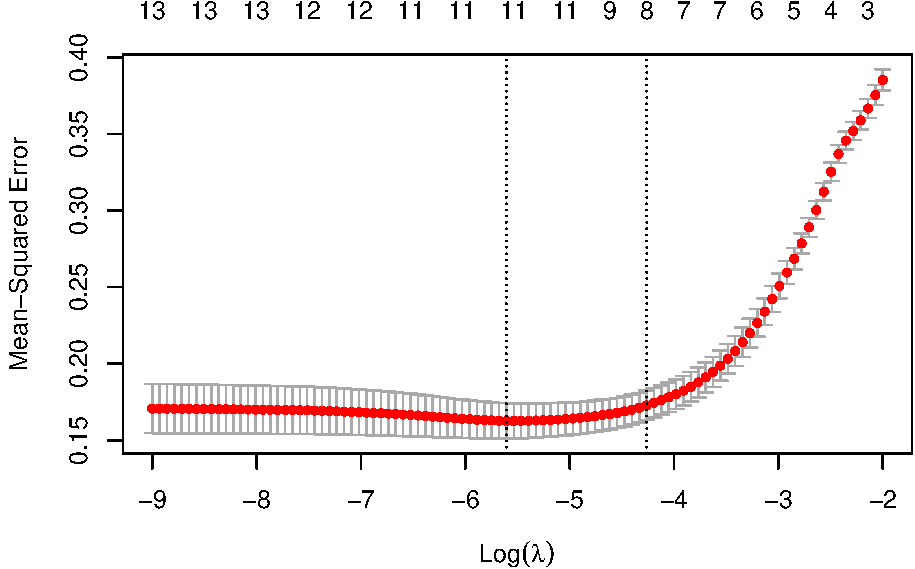
\includegraphics{Logistic-LASSO_files/figure-latex/unnamed-chunk-16-1.pdf}

\begin{Shaded}
\begin{Highlighting}[]
\NormalTok{cv.lasso}\OperatorTok{$}\NormalTok{lambda.min}
\end{Highlighting}
\end{Shaded}

\begin{verbatim}
## [1] 0.00367552
\end{verbatim}

\begin{Shaded}
\begin{Highlighting}[]
\KeywordTok{log}\NormalTok{(cv.lasso}\OperatorTok{$}\NormalTok{lambda.min)}
\end{Highlighting}
\end{Shaded}

\begin{verbatim}
## [1] -5.606061
\end{verbatim}

\begin{Shaded}
\begin{Highlighting}[]
\CommentTok{#coefficients}
\NormalTok{coeff =}\StringTok{ }\KeywordTok{coef}\NormalTok{(cv.lasso, }\DataTypeTok{s=}\NormalTok{cv.lasso}\OperatorTok{$}\NormalTok{lambda.min) }\OperatorTok\StringTok{ }\KeywordTok{as.numeric}\NormalTok{()}
\NormalTok{glmnet_coeff =}\StringTok{ }\KeywordTok{replace}\NormalTok{(coeff, }\KeywordTok{c}\NormalTok{(}\DecValTok{1}\NormalTok{,}\DecValTok{2}\OperatorTok{:}\DecValTok{14}\NormalTok{), coeff[}\KeywordTok{c}\NormalTok{(}\DecValTok{2}\OperatorTok{:}\DecValTok{14}\NormalTok{,}\DecValTok{1}\NormalTok{)])}

\CommentTok{#make tibble glmnet lasso coeff}
\NormalTok{glmnet_coeff_tib =}\StringTok{ }\KeywordTok{tibble}\NormalTok{(}\StringTok{`}\DataTypeTok{GLMnet}\StringTok{`}\NormalTok{ =}\StringTok{ }\KeywordTok{round}\NormalTok{(glmnet_coeff,}\DecValTok{4}\NormalTok{))}
\end{Highlighting}
\end{Shaded}

\subsubsection{Calculate MSE for Logistic-Lasso and Newton
Raphson}\label{calculate-mse-for-logistic-lasso-and-newton-raphson}

\begin{Shaded}
\begin{Highlighting}[]
\NormalTok{pred_error =}\StringTok{ }\ControlFlowTok{function}\NormalTok{(y, X, betavec) \{}
\NormalTok{  expu =}\StringTok{ }\KeywordTok{exp}\NormalTok{(}\KeywordTok{as.matrix}\NormalTok{(X) }\OperatorTok\StringTok{ }\NormalTok{betavec)}
\NormalTok{  p =}\StringTok{ }\NormalTok{expu}\OperatorTok{/}\NormalTok{(}\DecValTok{1}\OperatorTok{+}\NormalTok{expu)}
\NormalTok{  prediction_error =}\StringTok{ }\KeywordTok{mean}\NormalTok{((}\KeywordTok{as.vector}\NormalTok{(y)}\OperatorTok{-}\NormalTok{p)}\OperatorTok{^}\DecValTok{2}\NormalTok{)}
  \KeywordTok{return}\NormalTok{(prediction_error)}
\NormalTok{\}}
\end{Highlighting}
\end{Shaded}

\subsubsection{Newton Raphon's MSE}\label{newton-raphons-mse}

\begin{Shaded}
\begin{Highlighting}[]
\NormalTok{newton_raph_vec =}\StringTok{ }\NormalTok{newton_raph_res[}\KeywordTok{c}\NormalTok{(}\KeywordTok{nrow}\NormalTok{(newton_raph_res)),}\DecValTok{3}\OperatorTok{:}\KeywordTok{ncol}\NormalTok{(newton_raph_res)]}

\CommentTok{#nr_coeff_tib = tibble(`Newton-Raphson` = round(newton_raph_res[c(nrow(newton_raph_res)),3:ncol(newton_raph_res)]),4) }
\NormalTok{newton_raph_error =}\StringTok{ }\KeywordTok{pred_error}\NormalTok{(full_data}\OperatorTok{$}\NormalTok{diagnosis, Xmat_int, newton_raph_vec)}
\NormalTok{newton_raph_error}
\end{Highlighting}
\end{Shaded}

\begin{verbatim}
## [1] 0.07053378
\end{verbatim}

\subsubsection{Logistic-Lasso's MSE}\label{logistic-lassos-mse}

\begin{Shaded}
\begin{Highlighting}[]
\NormalTok{loglasso_betas =}\StringTok{ }\KeywordTok{coord.lasso}\NormalTok{(}\DataTypeTok{lambda =} \KeywordTok{as.numeric}\NormalTok{(best.ll.lambda), }
            \DataTypeTok{y =}\NormalTok{ full_data}\OperatorTok{$}\NormalTok{diagnosis, }
            \DataTypeTok{X =} \KeywordTok{as.matrix}\NormalTok{(Xmat_int), }
            \DataTypeTok{betavec =} \KeywordTok{rep}\NormalTok{(}\DecValTok{1}\NormalTok{, }\KeywordTok{ncol}\NormalTok{(Xmat_int)))}
\CommentTok{#get coefficients at best lambda }
\NormalTok{loglasso_betas =}\StringTok{ }\NormalTok{loglasso_betas[}\KeywordTok{nrow}\NormalTok{(loglasso_betas), }\DecValTok{3}\OperatorTok{:}\KeywordTok{ncol}\NormalTok{(loglasso_betas)]}

\CommentTok{#make tibble }
\NormalTok{loglasso_coeff_tib =}\StringTok{ }\KeywordTok{tibble}\NormalTok{(}\StringTok{`}\DataTypeTok{Logistic-LASSO}\StringTok{`}\NormalTok{ =}\StringTok{ }\KeywordTok{round}\NormalTok{(loglasso_betas, }\DecValTok{4}\NormalTok{))}

\CommentTok{#calc error}
\NormalTok{loglasso_error =}\StringTok{ }\KeywordTok{pred_error}\NormalTok{(full_data}\OperatorTok{$}\NormalTok{diagnosis, Xmat_int, loglasso_betas)}
\NormalTok{loglasso_error}
\end{Highlighting}
\end{Shaded}

\begin{verbatim}
## [1] 0.07272212
\end{verbatim}

GLMNet's MSE

\begin{Shaded}
\begin{Highlighting}[]
\NormalTok{glmnet_error =}\StringTok{ }\KeywordTok{pred_error}\NormalTok{(full_data}\OperatorTok{$}\NormalTok{diagnosis, Xmat_int, glmnet_coeff)}
\NormalTok{glmnet_error}
\end{Highlighting}
\end{Shaded}

\begin{verbatim}
## [1] 0.07193173
\end{verbatim}

\subsubsection{Summary table}\label{summary-table}

\begin{Shaded}
\begin{Highlighting}[]
\NormalTok{log_lasso =}\StringTok{ }\KeywordTok{c}\NormalTok{(}\DataTypeTok{error =} \KeywordTok{round}\NormalTok{(loglasso_error,}\DecValTok{4}\NormalTok{))}
\NormalTok{newton_raphson =}\StringTok{ }\KeywordTok{c}\NormalTok{(}\DataTypeTok{error =} \KeywordTok{round}\NormalTok{(newton_raph_error,}\DecValTok{4}\NormalTok{))}
\NormalTok{glmnet =}\StringTok{ }\KeywordTok{c}\NormalTok{(}\DataTypeTok{error =} \KeywordTok{round}\NormalTok{(glmnet_error,}\DecValTok{4}\NormalTok{))}

\NormalTok{table2 =}\StringTok{ }\KeywordTok{cbind}\NormalTok{(newton_raphson, log_lasso, glmnet)}

\KeywordTok{rownames}\NormalTok{(table2) <-}\StringTok{ }\KeywordTok{c}\NormalTok{(}\StringTok{"MSE"}\NormalTok{)}
\KeywordTok{colnames}\NormalTok{(table2)[}\DecValTok{1}\OperatorTok{:}\DecValTok{3}\NormalTok{] <-}\StringTok{ }\KeywordTok{c}\NormalTok{(}\StringTok{"Newton-Raphson"}\NormalTok{,}\StringTok{"Logistic LASSO"}\NormalTok{,}\StringTok{"GLMnet"}\NormalTok{) }
\NormalTok{knitr}\OperatorTok{::}\KeywordTok{kable}\NormalTok{(table2, }\DataTypeTok{escape =} \OtherTok{FALSE}\NormalTok{)}
\end{Highlighting}
\end{Shaded}

\begin{longtable}[]{@{}lrrr@{}}
\toprule
& Newton-Raphson & Logistic LASSO & GLMnet\tabularnewline
\midrule
\endhead
MSE & 0.0705 & 0.0727 & 0.0719\tabularnewline
\bottomrule
\end{longtable}

\subsubsection{Cross-validation}\label{cross-validation-1}

\begin{Shaded}
\begin{Highlighting}[]
\NormalTok{nr_mses =}\StringTok{ }\OtherTok{NULL}
\NormalTok{ll_mses =}\StringTok{ }\OtherTok{NULL}
\NormalTok{glmnet_mses =}\StringTok{ }\OtherTok{NULL}
\NormalTok{error_comp_df =}\StringTok{ }\OtherTok{NULL}
\KeywordTok{set.seed}\NormalTok{(}\DecValTok{2020}\NormalTok{)}

\CommentTok{#k-fold cross-validation}
\NormalTok{cv_comp =}\StringTok{ }\ControlFlowTok{function}\NormalTok{(X, y, fold_num)\{}
\NormalTok{  folds =}\StringTok{ }\KeywordTok{sample}\NormalTok{(}\DecValTok{1}\OperatorTok{:}\NormalTok{fold_num, }\KeywordTok{nrow}\NormalTok{(X), }\DataTypeTok{replace =} \OtherTok{TRUE}\NormalTok{)}
  \ControlFlowTok{for}\NormalTok{ (k }\ControlFlowTok{in} \DecValTok{1}\OperatorTok{:}\NormalTok{fold_num)\{}
  \CommentTok{#start = rep(1, ncol(X))}
\NormalTok{  x_train =}\StringTok{ }\KeywordTok{as.matrix}\NormalTok{(X[folds }\OperatorTok{!=}\StringTok{ }\NormalTok{k,])}
\NormalTok{  y_train =}\StringTok{ }\NormalTok{y[folds }\OperatorTok{!=}\StringTok{ }\NormalTok{k] }
\NormalTok{  x_test =}\StringTok{ }\KeywordTok{as.matrix}\NormalTok{(X[folds }\OperatorTok{==}\StringTok{ }\NormalTok{k,]) }
\NormalTok{  y_test =}\StringTok{ }\NormalTok{y[folds }\OperatorTok{==}\StringTok{ }\NormalTok{k]}
  
\NormalTok{  ll_expu =}\StringTok{ }\KeywordTok{exp}\NormalTok{(x_test }\OperatorTok\StringTok{ }\NormalTok{loglasso_betas)}
\NormalTok{  ll_p =}\StringTok{ }\NormalTok{ll_expu}\OperatorTok{/}\NormalTok{(}\DecValTok{1}\OperatorTok{+}\NormalTok{ll_expu)}
\NormalTok{  ll_mse =}\StringTok{ }\KeywordTok{mean}\NormalTok{((y_test}\OperatorTok{-}\NormalTok{ll_p)}\OperatorTok{^}\DecValTok{2}\NormalTok{) }\CommentTok{#cross-validated MSE for logistic lasso}
\NormalTok{  ll_mses =}\StringTok{ }\KeywordTok{rbind}\NormalTok{(ll_mses, ll_mse)}
  
\NormalTok{  nr_expu =}\StringTok{ }\KeywordTok{exp}\NormalTok{(x_test }\OperatorTok\StringTok{ }\NormalTok{newton_raph_vec)}
\NormalTok{  nr_p =}\StringTok{ }\NormalTok{nr_expu}\OperatorTok{/}\NormalTok{(}\DecValTok{1}\OperatorTok{+}\NormalTok{nr_expu)}
\NormalTok{  nr_mse =}\StringTok{ }\KeywordTok{mean}\NormalTok{((y_test }\OperatorTok{-}\StringTok{ }\NormalTok{nr_p)}\OperatorTok{^}\DecValTok{2}\NormalTok{) }\CommentTok{#cross-validated MSE for newton-raphson}
\NormalTok{  nr_mses =}\StringTok{ }\KeywordTok{rbind}\NormalTok{(nr_mses, nr_mse)}
  
\NormalTok{  glmnet_expu =}\StringTok{ }\KeywordTok{exp}\NormalTok{(x_test }\OperatorTok\StringTok{ }\NormalTok{glmnet_coeff)}
\NormalTok{  glmnet_p =}\StringTok{ }\NormalTok{glmnet_expu}\OperatorTok{/}\NormalTok{(}\DecValTok{1}\OperatorTok{+}\NormalTok{glmnet_expu)}
\NormalTok{  glmnet_mse =}\StringTok{ }\KeywordTok{mean}\NormalTok{((y_test }\OperatorTok{-}\StringTok{ }\NormalTok{glmnet_p)}\OperatorTok{^}\DecValTok{2}\NormalTok{) }\CommentTok{#cross-validated MSE for glmnet}
\NormalTok{  glmnet_mses =}\StringTok{ }\KeywordTok{rbind}\NormalTok{(glmnet_mses, glmnet_mse)}
\NormalTok{  \}}
\NormalTok{  res =}\StringTok{ }\KeywordTok{tibble}\NormalTok{(}\StringTok{`}\DataTypeTok{GLMnet}\StringTok{`}\NormalTok{=}\StringTok{ }\NormalTok{glmnet_mse, }\StringTok{`}\DataTypeTok{Logistic-LASSO}\StringTok{`}\NormalTok{ =}\StringTok{ }\NormalTok{ll_mses, }\StringTok{`}\DataTypeTok{Newton-Raphson}\StringTok{`}\NormalTok{ =}\StringTok{ }\NormalTok{nr_mses)}
  \KeywordTok{return}\NormalTok{(res)\}}

\CommentTok{#repeated cross-validation n times}
\NormalTok{rep_cv =}\StringTok{ }\ControlFlowTok{function}\NormalTok{(X, y, fold_num, n)\{}
  \ControlFlowTok{while}\NormalTok{ (i }\OperatorTok{<=}\StringTok{ }\NormalTok{n)\{}
\NormalTok{    i =}\StringTok{ }\NormalTok{i}\OperatorTok{+}\DecValTok{1}
\NormalTok{    error_comp =}\StringTok{ }\KeywordTok{cv_comp}\NormalTok{(X, y, fold_num)}
\NormalTok{    error_comp_df =}\StringTok{ }\KeywordTok{rbind}\NormalTok{(error_comp_df, error_comp)}
\NormalTok{  \}}
  \KeywordTok{return}\NormalTok{(error_comp_df)}
\NormalTok{\}}

\NormalTok{mse_comp_df =}\StringTok{ }\KeywordTok{rep_cv}\NormalTok{(}\DataTypeTok{X =}\NormalTok{ Xmat_int, }\DataTypeTok{y =}\NormalTok{ full_data}\OperatorTok{$}\NormalTok{diagnosis, }\DataTypeTok{fold_num =} \DecValTok{5}\NormalTok{, }\DataTypeTok{n =}\DecValTok{1}\NormalTok{)}

\NormalTok{rep_mse_comp_df =}\StringTok{ }\KeywordTok{rep_cv}\NormalTok{(}\DataTypeTok{X =}\NormalTok{ Xmat_int, }\DataTypeTok{y =}\NormalTok{ full_data}\OperatorTok{$}\NormalTok{diagnosis, }\DataTypeTok{fold_num =} \DecValTok{5}\NormalTok{, }\DataTypeTok{n =}\DecValTok{5}\NormalTok{)}
\end{Highlighting}
\end{Shaded}

\subsubsection{Visualize error
comparisons}\label{visualize-error-comparisons}

\begin{Shaded}
\begin{Highlighting}[]
\NormalTok{mse_comp_df }\OperatorTok\StringTok{ }
\StringTok{  }\KeywordTok{pivot_longer}\NormalTok{(}\DecValTok{1}\OperatorTok{:}\DecValTok{3}\NormalTok{, }\DataTypeTok{names_to =} \StringTok{"Model"}\NormalTok{, }\DataTypeTok{values_to =} \StringTok{"MSE"}\NormalTok{) }\OperatorTok\StringTok{ }
\StringTok{  }\KeywordTok{ggplot}\NormalTok{(}\KeywordTok{aes}\NormalTok{(}\DataTypeTok{x =}\NormalTok{ MSE, }\DataTypeTok{col =}\NormalTok{ Model, }\DataTypeTok{fill =}\NormalTok{ Model)) }\OperatorTok{+}\StringTok{ }
\StringTok{  }\KeywordTok{geom_density}\NormalTok{(}\DataTypeTok{adjust =} \FloatTok{1.5}\NormalTok{, }\DataTypeTok{alpha =} \FloatTok{0.3}\NormalTok{) }\OperatorTok{+}\StringTok{ }
\StringTok{  }\KeywordTok{labs}\NormalTok{(}\DataTypeTok{title =} \StringTok{"Distribution of 5-fold cross-validated MSE across models"}\NormalTok{,}
       \DataTypeTok{x =} \StringTok{"Cross-validated MSE"}\NormalTok{,}
       \DataTypeTok{y =} \StringTok{"Density"}\NormalTok{) }\OperatorTok{+}
\StringTok{  }\KeywordTok{theme}\NormalTok{(}\DataTypeTok{legend.position =} \StringTok{"bottom"}\NormalTok{,}
        \DataTypeTok{plot.title =} \KeywordTok{element_text}\NormalTok{(}\DataTypeTok{size=} \DecValTok{11}\NormalTok{, }\DataTypeTok{hjust =} \FloatTok{0.5}\NormalTok{))}
\end{Highlighting}
\end{Shaded}

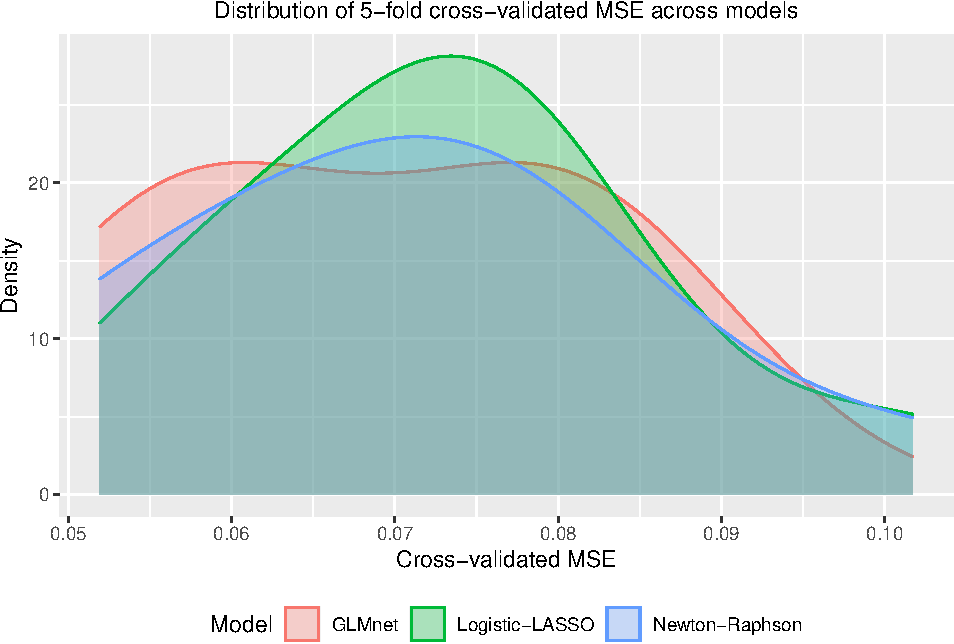
\includegraphics{Logistic-LASSO_files/figure-latex/unnamed-chunk-23-1.pdf}

\begin{Shaded}
\begin{Highlighting}[]
\NormalTok{rep_mse_comp_df }\OperatorTok\StringTok{ }
\StringTok{  }\KeywordTok{pivot_longer}\NormalTok{(}\DecValTok{1}\OperatorTok{:}\DecValTok{3}\NormalTok{, }\DataTypeTok{names_to =} \StringTok{"Model"}\NormalTok{, }\DataTypeTok{values_to =} \StringTok{"MSE"}\NormalTok{) }\OperatorTok\StringTok{ }
\StringTok{  }\KeywordTok{ggplot}\NormalTok{(}\KeywordTok{aes}\NormalTok{(}\DataTypeTok{x =}\NormalTok{ MSE, }\DataTypeTok{col =}\NormalTok{ Model, }\DataTypeTok{fill =}\NormalTok{ Model)) }\OperatorTok{+}\StringTok{ }
\StringTok{  }\KeywordTok{geom_density}\NormalTok{(}\DataTypeTok{adjust =} \FloatTok{1.5}\NormalTok{, }\DataTypeTok{alpha =} \FloatTok{0.3}\NormalTok{) }\OperatorTok{+}\StringTok{ }
\StringTok{  }\KeywordTok{labs}\NormalTok{(}\DataTypeTok{title =} \StringTok{"Distribution of repeated 5-fold cross-validated MSE across models"}\NormalTok{,}
       \DataTypeTok{x =} \StringTok{"Cross-validated MSE"}\NormalTok{,}
       \DataTypeTok{y =} \StringTok{"Density"}\NormalTok{) }\OperatorTok{+}
\StringTok{  }\KeywordTok{theme}\NormalTok{(}\DataTypeTok{legend.position =} \StringTok{"bottom"}\NormalTok{,}
        \DataTypeTok{plot.title =} \KeywordTok{element_text}\NormalTok{(}\DataTypeTok{size=} \DecValTok{11}\NormalTok{, }\DataTypeTok{hjust =} \FloatTok{0.5}\NormalTok{))}
\end{Highlighting}
\end{Shaded}

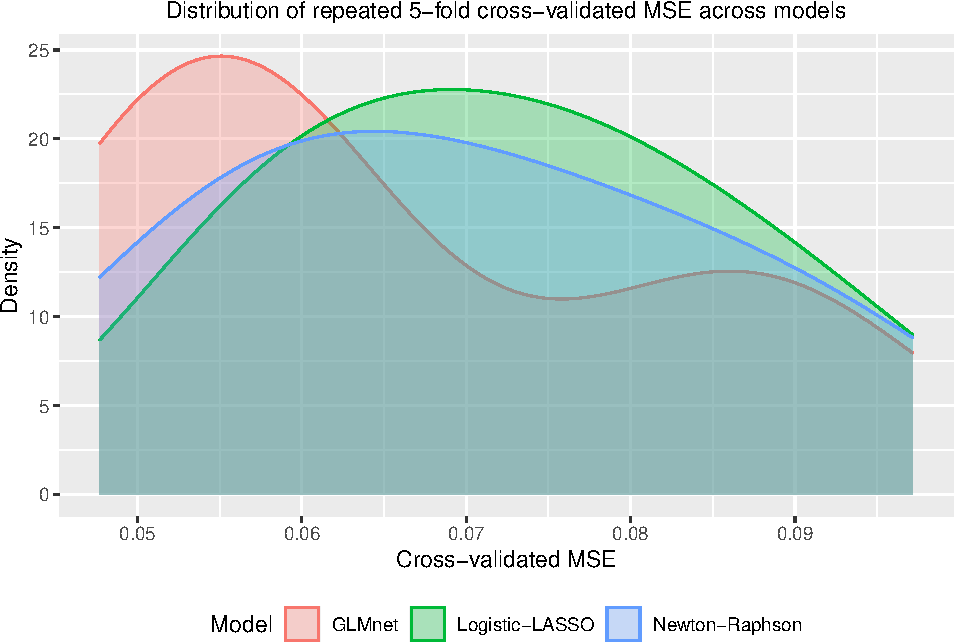
\includegraphics{Logistic-LASSO_files/figure-latex/unnamed-chunk-23-2.pdf}

\subsubsection{All coefficients by all
model}\label{all-coefficients-by-all-model}

\begin{Shaded}
\begin{Highlighting}[]
\NormalTok{table1 =}\StringTok{ }\KeywordTok{cbind}\NormalTok{(glm_coeff_tib, }\KeywordTok{t}\NormalTok{(nr_coeff_tib), glmnet_coeff_tib, loglasso_coeff_tib) }\OperatorTok\StringTok{ }\KeywordTok{rename_at}\NormalTok{(}\DecValTok{2}\NormalTok{, }\OperatorTok{~}\StringTok{"Newton-Raphson"}\NormalTok{)}

\NormalTok{knitr}\OperatorTok{::}\KeywordTok{kable}\NormalTok{(table1, }\DataTypeTok{escape =} \OtherTok{FALSE}\NormalTok{)}
\end{Highlighting}
\end{Shaded}

\begin{longtable}[]{@{}lrrrr@{}}
\toprule
& GLM binomial & Newton-Raphson & GLMnet & Logistic-LASSO\tabularnewline
\midrule
\endhead
smoothness\_mean & 1.5725 & 1.5725 & 1.1176 & 1.0229\tabularnewline
symmetry\_mean & -0.1187 & -0.1187 & 0.0000 & 0.0000\tabularnewline
fractal\_dimension\_mean & -4.5061 & -4.5061 & -3.5738 &
-3.3703\tabularnewline
texture\_se & 0.8068 & 0.8068 & 0.5009 & 0.4466\tabularnewline
smoothness\_se & -0.8304 & -0.8304 & -0.6757 & -0.6253\tabularnewline
compactness\_se & 0.3954 & 0.3954 & 0.1787 & 0.1392\tabularnewline
concavity\_se & -0.0300 & -0.0300 & 0.0000 & 0.0000\tabularnewline
concave.points\_se & 2.2856 & 2.2856 & 1.8469 & 1.7472\tabularnewline
symmetry\_se & -0.2039 & -0.2039 & -0.0997 & -0.0615\tabularnewline
fractal\_dimension\_se & -0.7551 & -0.7551 & -0.3363 &
-0.2821\tabularnewline
smoothness\_worst & 0.7859 & 0.7859 & 0.8685 & 0.8577\tabularnewline
symmetry\_worst & 1.0091 & 1.0091 & 0.7511 & 0.7050\tabularnewline
fractal\_dimension\_worst & 2.8346 & 2.8346 & 2.1066 &
1.9924\tabularnewline
intercept & -1.5278 & -1.5278 & -1.2742 & -1.1624\tabularnewline
\bottomrule
\end{longtable}

\subsubsection{ROC curves}\label{roc-curves}

\begin{Shaded}
\begin{Highlighting}[]
\NormalTok{nr_pred_prob <-}\StringTok{ }\KeywordTok{predict}\NormalTok{(log.mod, }\DataTypeTok{newdata =}\NormalTok{ full_data, }\DataTypeTok{type =} \StringTok{"response"}\NormalTok{)}

\NormalTok{roc.glm <-}\StringTok{ }\KeywordTok{roc}\NormalTok{(full_data}\OperatorTok{$}\NormalTok{diagnosis, nr_pred_prob)}
\KeywordTok{plot}\NormalTok{(roc.glm, }\DataTypeTok{legacy.axes =} \OtherTok{TRUE}\NormalTok{, }\DataTypeTok{print.auc =} \OtherTok{TRUE}\NormalTok{)}
\end{Highlighting}
\end{Shaded}

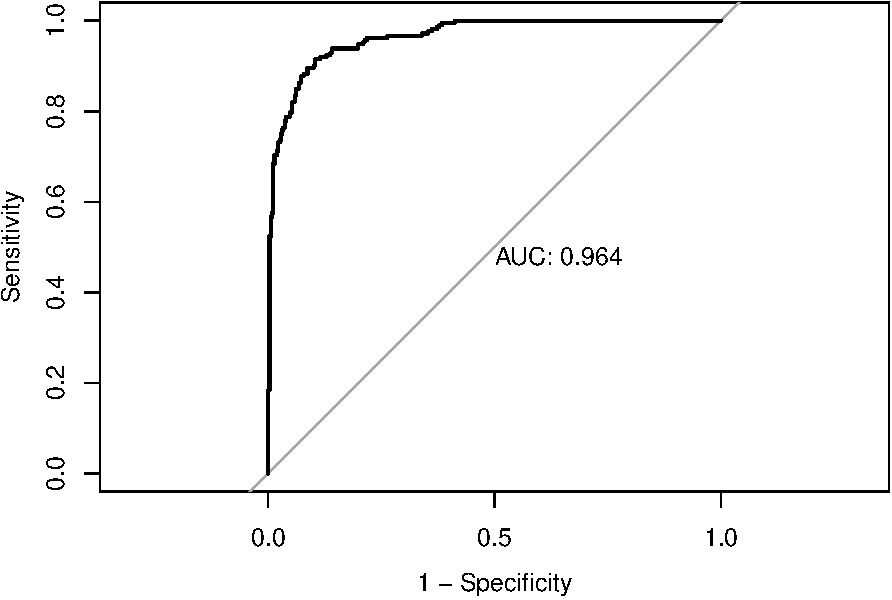
\includegraphics{Logistic-LASSO_files/figure-latex/unnamed-chunk-25-1.pdf}

\end{document}
